\def\CTeXPreproc{Created by ctex v0.2.9, don't edit!}
%\documentclass{beamer}
\documentclass[%handout,
xcolor=pdftex]{beamer}
\mode<presentation> {
  \usetheme{Warsaw}
  \setbeamercovered{transparent}
}
\let\Tiny=\tiny
\usetheme{Singapore}
\usecolortheme{dolphin}
\usepackage{amsmath}
\usepackage{textcomp}
\usepackage{amssymb}
\usepackage{amsthm}
\usepackage{graphicx}
\usepackage{color}
\usepackage{lipsum}
\usepackage{hyperref}
\usepackage{multirow}
\usepackage{bm}
%\setbeamertemplate{headline}{}
\setbeamertemplate{footline}[page number]
\newcommand\Fontvi{\fontsize{9pt}{8}\selectfont}
\newcommand\Fontvii{\fontsize{7pt}{8}\selectfont}
\newcommand{\backupbegin}{
   \newcounter{finalframe}
   \setcounter{finalframe}{\value{framenumber}}
}
\newcommand{\backupend}{
   \setcounter{framenumber}{\value{finalframe}}
}\newtheorem{proposition}{Proposition}
\title{Unit 11: ARMA Autocorrelation and Partial Autocorrelation Functions}
\author[STAT 5170: Applied Time Series, Unit 11]{Taylor R. Brown}
\institute{Department of Statistics, University of Virginia}
\date{Fall 2020}

\AtBeginSubsection[] {
  \begin{frame}<beamer>{Outline}
    \tableofcontents[currentsection,currentsubsection]
  \end{frame}
}

\begin{document}


\frame{\titlepage}


\begin{frame}
\frametitle{Readings for Unit 11}

Textbook chapter 3.3.

\end{frame}


\begin{frame}
\frametitle{Last Unit}
\begin{enumerate}
\item ARMA(p,q)
\item Condition for causality
\item Condition for invertibility
\item Condition for redundant parameters (shared roots)
\end{enumerate}
\end{frame}


\begin{frame}
\frametitle{This Unit}
\begin{enumerate}
\item ACF for MA(q)
\item ACF for Causal ARMA(p,q)
\item Partial Autocorrelation Function (PACF)
\end{enumerate}
\end{frame}


\begin{frame}
\frametitle{Motivation}

In this unit we will study the autocorrelation and partial autocorrelation
 functions for ARMA processes.

\end{frame}

\section{ACF for MA(q) Processes}
%\frame{\tableofcontents[currentsection]}

\begin{frame}
\frametitle{MA(q) Process}

 Let's start with an MA($q$) process
 $$
 x_t = w_t + \theta_1 w_{t-1} + \theta_2 w_{t-2} + \cdots + \theta_q w_{t-q} = \sum^q_{j=0} \theta_j w_{t-j},
 $$
where we have written $\theta_0=1$. Then
$$
E(x_t) =\sum^q_{j=0} \theta_j E(w_{t-j})=0.
$$

\end{frame}

\begin{frame}
\frametitle{Autocovariance for MA(q)}

The autocovariance function is
\begin{eqnarray*}
\gamma(h) = cov(x_t,x_{t+h}) &=& E \Big [ \sum^q_{j=0} \theta_j w_{t-j} \sum^q_{j'=0} \theta_{j'} w_{t+h-j'} \Big ] \cr
&=& \sum^q_{j=0} \sum^q_{j'=0} \theta_j \theta_{j'} E(w_{t-j} w_{t+h-j'}).
\end{eqnarray*}

\end{frame}

\begin{frame}
\frametitle{Autocovariance for MA(q)}

Recall that $E(w_s w_t) = \sigma^2_w$ if $s=t$ and $E(w_s
w_t)=0$ otherwise. So we have
\begin{eqnarray}\label{eq:1}
\gamma(h) = \left \{ \begin{array}{ll}
\sigma^2_w \sum^{q-h}_{j=0} \theta_j \theta_{j+h}, & 0 \le h\le q, \\
0, & h \ge q+1.
\end{array} \right.
\end{eqnarray}


\end{frame}

\begin{frame}
\frametitle{ACF for MA(q)}

Recall that $\gamma(h)=\gamma(-h)$, so we will only need the
values for $h\ge 0$. Dividing $\gamma(h)$ by $\gamma(0)$ in
(\ref{eq:1}), we obtain the autocorrelation function (ACF) of
an MA($q$) model
\begin{eqnarray}\label{eq:2}
\rho(h) = \left \{ \begin{array}{ll}
\frac{\sum^{q-h}_{j=0} \theta_j \theta_{j+h}}{1+\theta^2_1+\cdots+\theta^2_q}, & 0 \le h\le q, \\
0, & h \ge q+1.
\end{array} \right.
\end{eqnarray}


\end{frame}

\section{ACF for Causal ARMA(p,q) Processes}
\frame{\tableofcontents[currentsection]}

\begin{frame}
\frametitle{ACF for Causal ARMA(p,q)}

We have seen in (\ref{eq:2}), for MA($q$) models, the ACF will
be zero for lags greater than $q$. Moreover, because
$\theta_q\ne 0$,
$\rho(q)=\theta_0\theta_q/(1+\theta_1^2+\cdots+\theta^2_q)\ne
0$. Thus, the ACF provides information
about the order of the dependence for a MA model. How about
ARMA or AR models?

\end{frame}

\begin{frame}
\frametitle{Causal ARMA(p,q)}

Now we discuss causal ARMA($p,q$) model
$$
\phi(B) x_t = \theta(B) w_t,
$$
where the roots of $\phi(z)$ are outside the unit circle. Ths means for $|z| \le 1$, $|\phi(z)| > 0$, which means $|\phi^{-1}(z)| < \infty$. 
\newline

We have the MA($\infty$) representation
\begin{eqnarray}\label{eq:3}
x_t = \sum^\infty_{j=0} \psi_j w_{t-j},  \quad \mbox{where} \quad
\psi(z) = \frac{\theta(z)}{\phi(z)} = \sum^\infty_{j=0} \psi_j z^j.
\end{eqnarray}

\end{frame}

\begin{frame}
\frametitle{Autocovariance for Causal ARMA(p,q)}

It follows  that $E(x_t)=0$ and by (\ref{eq:1}), the
autocovariance function of $x_t$ is given by
$$
\gamma(h) =cov(x_t,x_{t+h})= \sigma^2_w \sum^\infty_{j=0} \psi_j \psi_{j+h},
\quad h\ge 0.
$$

\end{frame}

\begin{frame}
\frametitle{Autocovariance for Causal ARMA(p,q)}

We won't provide an explicit formula for the ACF of an ARMA(p,q), but we will derive the system of equations you'll need to solve to get it. 
%\newline

Let $h\ge 0$, and $\theta_0 = 1$:
\begin{align*}
\gamma_X(h) &= \text{Cov}(X_{t+h}, X_t) \\
&= \text{Cov}(\sum_{i=1}^p \phi_i X_{t+h-i} + \sum_{j=0}^q \theta_j W_{t+h-j}, X_t)\\
&= \sum_{i=1}^p \phi_i \text{Cov}(X_{t+h-i} , X_t) + \sum_{j=0}^q \theta_j \text{Cov}\left( W_{t+h-j}, X_t\right) \\
&= \sum_{i=1}^p \phi_i \gamma_X(h-i) + \sum_{j=0}^q \theta_j \text{Cov}\left( W_{t+h-j}, \sum^\infty_{k=0} \psi_k W_{t-k}\right)
\end{align*}

\end{frame}


\begin{frame}
\frametitle{ACVF and ACF for Causal ARMA(p,q)}

Let $h\ge 0$, and $\theta_0 = 1$:
\begin{align*}
\gamma_X(h) &= \sum_{i=1}^p \phi_i \gamma_X(h-i) + \sum_{j=0}^q \theta_j \text{Cov}\left( W_{t+h-j}, \sum^\infty_{k=0} \psi_k W_{t-k}\right) \\
&= \sum_{i=1}^p \phi_i \gamma_X(h-i) + \sum_{j=0}^q\sum^\infty_{k=0}  \theta_j\psi_k \sigma^2_W 1( t+h-j = t-k) \\
&= \sum_{i=1}^p \phi_i \gamma_X(h-i) + \sigma^2_W \sum_{j=h}^q \theta_j\psi_{j-h} 
\end{align*}

$0 \le j < \infty$, $k \ge 0$, and $k = j - h$. Dividing through by $\gamma(0)$ will give the equations for solving $\rho(\cdot)$.

\end{frame}

\begin{frame}
\frametitle{ACVF and ACF for Causal ARMA(1,1)}

For a causal ARMA(p,q), $h\ge 0$, :
$$
\gamma_X(h) = \sum_{i=1}^p \phi_i \gamma_X(h-i) + \sigma^2_W \sum_{j=h}^q \theta_j\psi_{j-h} 
$$

Let's consider an ARMA(1,1). When $h \ge 2$, we have
$$
\gamma(h) = \phi_1 \gamma_X(h-1)
$$
This means $\gamma(h) = \phi_1^h c$ for some unknown $c \in \mathbb{R}$. To find $c$ we consider the ``initial conditions" or when $h = 0,1$.

\end{frame}


\begin{frame}
\frametitle{ACVF and ACF for Causal ARMA(1,1)}

For a causal ARMA(p,q), $h\ge 0$, :
$$
\gamma_X(h) = \sum_{i=1}^p \phi_i \gamma_X(h-i) + \sigma^2_W \sum_{j=h}^q \theta_j\psi_{j-h} 
$$

Still considering an ARMA(1,1), when $h = 0,1$, we have
\begin{eqnarray}
\gamma(0) = \phi_1 \gamma(-1) + \sigma^2_W\sum_{j=0}^1 \theta_j \psi_{j} \\
\gamma(1) = \phi_1 \gamma(0)  + \sigma^2_W \theta_1 
\end{eqnarray}

This yields (dropping the subscripts from $\theta_1$ and $\phi_1$)
$$
\rho(h) = \frac{(1 + \theta\phi)(\phi + \theta)}{(1 + 2 \theta\phi + \theta^2)}\phi^{h-1}
$$
Notice that there is only one part dependent on $h$!

\end{frame}


\begin{frame}
\frametitle{ACVF for Causal AR(1)}

For a causal ACVF,
$$
\gamma_X(h) = \sum_{i=1}^p \phi_i \gamma_X(h-i) + \sigma^2_W \sum_{j=h}^q \theta_j\psi_{j-h} 
$$

Consider a causal AR(P) model $x_t=\phi_1
x_{t-1}+w_t$.  Then

$$
\gamma_X(h) = \sum_{i=1}^p \phi_i \gamma_X(h-i) 
$$

$\gamma_X(h)$ will never cut-off to $0$ for any $h$. This makes it difficult to identify what $p$ is.


\vspace{40mm}

\end{frame}

\begin{frame}
\frametitle{A new idea for causal AR(p) models}

We'll need this trick in the following slide...
\newline

Note we can write $X_t = \sum_{i=0}^{\infty} \psi_i W_{t-i}$
\newline

Causality means $x_{t-2}$, for example, only depends on $w_{t-2},w_{t-3},\ldots$ and hence is uncorrelated with $w_{t-1}$ and $w_t$. 

For $s > t$, check $\text{Cov}(w_{s},x_{t})= \sum_{i=0}^{\infty} \psi_j \overbrace{\text{Cov}(w_{s},w_{t-i})}^{0}$. 

\end{frame}


\begin{frame}
\frametitle{A new idea for causal AR(p) models}

For a causal AR(1) model, the $\gamma_X$ and $\rho_X$ functions don't zero out past $p$, so instead consider 
\begin{align*}
\text{Cov}(x_{t+2} - \hat{x}_{t+2},x_{t} - \hat{x}_t) &= \text{Cov}(x_{t+2} - \phi x_{t+1},x_{t} - \phi x_{t+1}) \\
&= \text{Cov}(w_{t+2}, x_{t} - \phi x_{t+1}) \\
&= \text{Cov}(w_{t+2}, x_{t}) - \phi \text{Cov}(w_{t+2}, x_{t+1}) \\
&= 0
\end{align*}

So, when considering the relationship between $x_{t+2}$ and $x_t$, we first remove the linear dependence on $x_{t+1}$!

\end{frame}

\begin{frame}
\frametitle{Notation}

One way to remove linear connections is through \textbf{linear
regression}. 
\newline

Let $\hat{x}_{t+h}$ denote the regression of $x_{t+h}$ on
$\{x_{t+h-1},x_{t+h-2},\ldots,x_{t+1}\}$, which we write as
\begin{equation}
\hat{x}_{t+h} = \beta_1 x_{t+h-1} + \beta_2 x_{t+h-2} + \cdots + \beta_{h-1} x_{t+1}.
\end{equation}
Here we do not include the intercept assuming the mean of $x_t$
is zero. Otherwise, replace $x_t$ with $x_t - \mu_x$.

\end{frame}

\begin{frame}
\frametitle{Notation}

In addition, let $\hat{x}_t$ denote the regression of
$x_t$ on $\{x_{t+1},x_{t+2},\ldots,x_{t+h-1}\}$, then
\begin{equation}
\hat{x}_t = \beta_1 x_{t+1} + \beta_2 x_{t+2} + \cdots + \beta_{h-1} x_{t+h-1}.
\end{equation}

\end{frame}

\section{Partial Autocorrelation Function}
\frame{\tableofcontents[currentsection]}

\begin{frame}
\frametitle{Partial Autocorrelation Function}

The {\bf partial autocorrelation
function (PACF)} of a stationary process $x_t$, denoted by
$\phi_{hh}$, for $h=1,2,\ldots$, is

\begin{equation}
\phi_{11} = corr(x_{t+1},x_t) = \rho(1)
\end{equation}
and
\begin{equation}
\phi_{hh}=corr(x_{t+h}-\hat{x}_{t+h}, x_t-\hat{x}_t), \quad h\ge 2.
\end{equation}

Note that, the PACF, $\phi_{hh}$ is the correlation between
$x_{t+h}$ and $x_{t}$ with the linear dependence of
$\{x_{t+1},\cdots,x_{t+h-1}\}$, on each, removed.

\end{frame}

\begin{frame}


\frametitle{Partial Autocorrelation Function: AR(1) example}

Let's go back to the example from a few slides ago, and try to calculate the PACF of a causal AR(1) model: $x_t=\phi
x_{t-1}+w_t$, with $|\phi|<1$.
\newline

By definition, $\phi_{11}=corr(x_1,x_0)=\rho(1)=\phi$. 
\newline

We wrote
\begin{align*}
\phi_{22} &:= \text{Cov}(x_{t+2} - \hat{x}_{t+2},x_{t} - \hat{x}_t) \\
&= 0
\end{align*}

...but why are $\hat{x}_{t+2} = \hat{x}_t = \phi x_{t+1}$? 

\end{frame}


\begin{frame}
\frametitle{Partial Autocorrelation Function: AR(1) example}

To calculate $\phi_{22}$, consider the regression of $x_{t+2}$ on $x_{t+1}$, say $\hat{x}_{t+2}=\beta x_{t+1}$.
\newline

We choose $\beta$ to minimize 
$$
E\left[ \left( x_{t+2} - \beta x_{t+1}\right)^2 \right] = \gamma_X(0) - 2\beta \gamma_X(1) + \beta^2 \gamma_X(0).
$$

Taking the derivative and setting that equal to $0$ yields $\beta = \phi$.

\end{frame}



\begin{frame}
\frametitle{Partial Autocorrelation Function}

Next, consider the regression of $x_t$ on $x_{t+1}$, say
$\hat{x}_t=\beta x_{t+1}$. We choose $\beta$ to minimize

\vspace{50mm}

\end{frame}

\begin{frame}
\frametitle{Partial Autocorrelation Function}

In general, for a causal AR($p$) model $x_h=\sum^p_{j=1}\phi_j
x_{h-j}+w_h$. When $h>p$, the regression of $x_h$ on
$x_{h-1},\ldots,x_1$ is
$$
\hat{x}_{h} = \sum^p_{j=1} \phi_j x_{h-j}.
$$

\end{frame}

\begin{frame}
\frametitle{Partial Autocorrelation Function}

Thus, when $h>p$, by causality,
$$
\phi_{hh} = corr(x_h-\hat{x}_{h},x_0-\hat{x}_{0}) = corr(w_h,x_0-\hat{x}_{0}) = 0.
$$

\end{frame}

\begin{frame}
\frametitle{Summary}

\begin{itemize}
\item The ACF of MA($q$) model cuts off after lag $q$. The PACF of an AR($p$) model cuts off after lag $p$.
\item Identification of an MA(q) model is best done with ACF; identification of an AR(p) model is best done with PACF.
\item The PACF between $x_t$ and $x_{t-h}$ is the correlation between $x_t - \hat{x}_t$ and $x_{t-h} - \hat{x}_{t-h}$. Think of it as taking the correlation between the residuals from two regression models. The dependence on all intermediate variables is removed. 
\end{itemize}

\end{frame}

\section{Worked Examples}
\frame{\tableofcontents[currentsection]}

\begin{frame}
\frametitle{ACF and PACF of Causal AR(2)}

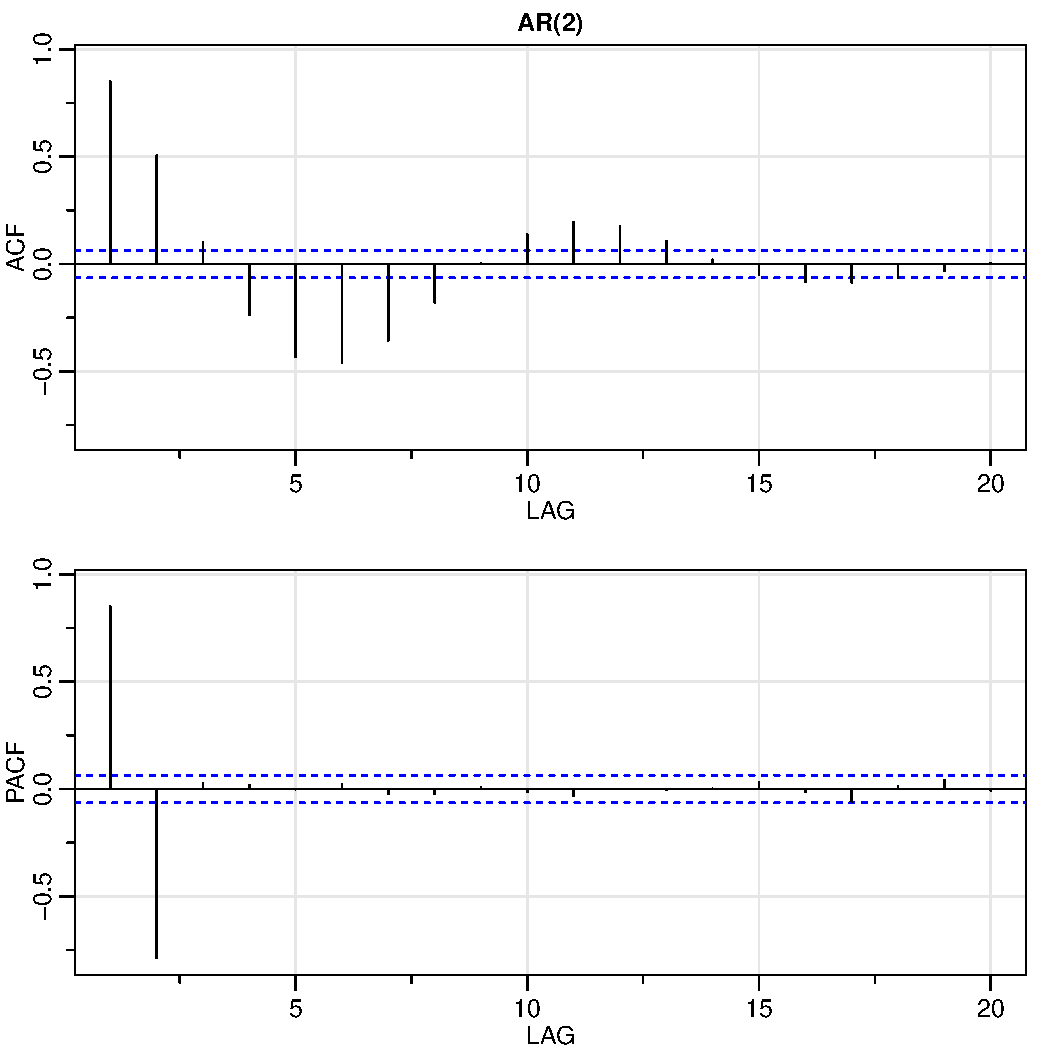
\includegraphics[width=100mm, height=80mm]{ar.pdf}

\end{frame}

\begin{frame}
\frametitle{ACF and PACF of Invertible MA(2)}

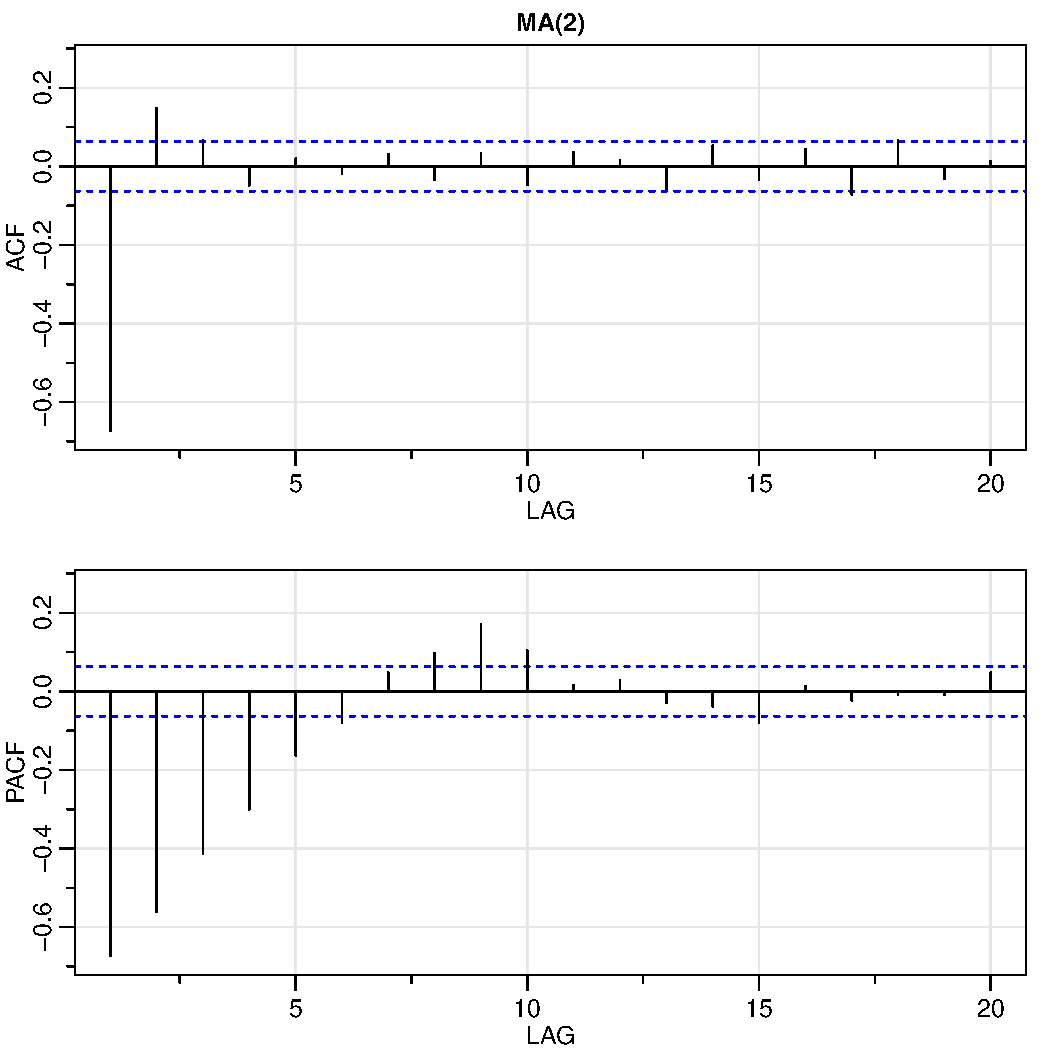
\includegraphics[width=100mm, height=80mm]{ma.pdf}

\end{frame}

\begin{frame}
\frametitle{ACF and PACF of Causal and Invertible ARMA(2,2)}

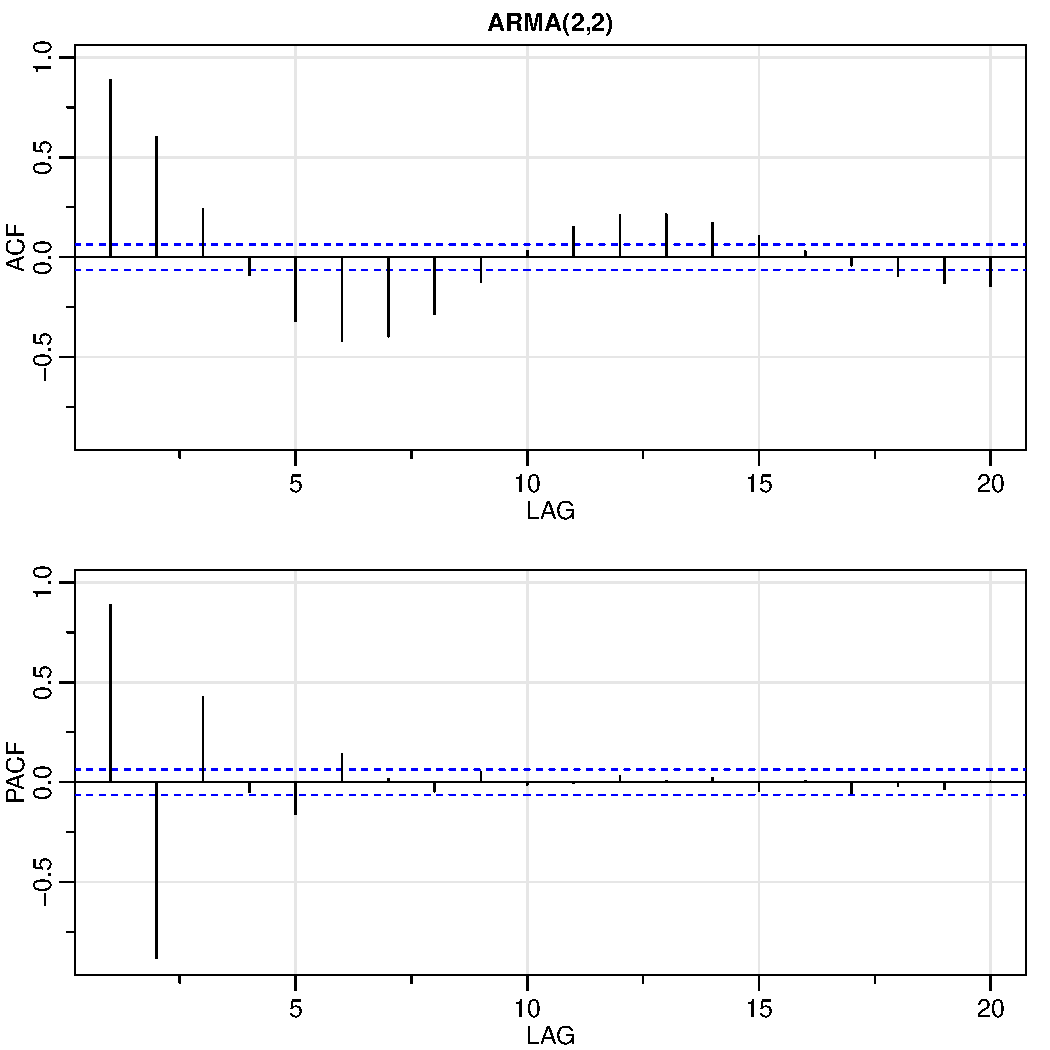
\includegraphics[width=100mm, height=80mm]{arma.pdf}

\end{frame}

\begin{frame}
\frametitle{ACF and PACF of Causal AR and Invertible MA}

(From page 99, Table 3.1 of text)

\begin{center}
\begin{tabular}{cccc}
\hline \\
 & \textbf{AR(p)} & \textbf{MA(q)} & \textbf{ARMA(p,q)} \\
\hline \\
ACF & Decay & 0 after lag $q$ & Decay\\
PACF & 0 after lag $p$ & Decay & Decay\\
\hline
\end{tabular}
\end{center}

\end{frame}

\begin{frame}
\frametitle{Fish Population Example}

This time series from ``recruit.dat" contains data on fish population in the central Pacific Ocean. The numbers represent the number of new fish in the years 1950-1987. \textbf{Question}: Based on the ACF and PACF plots, what process do you think is most likely to describe this time series?

\end{frame}

\begin{frame}
\frametitle{Fish Population Example}

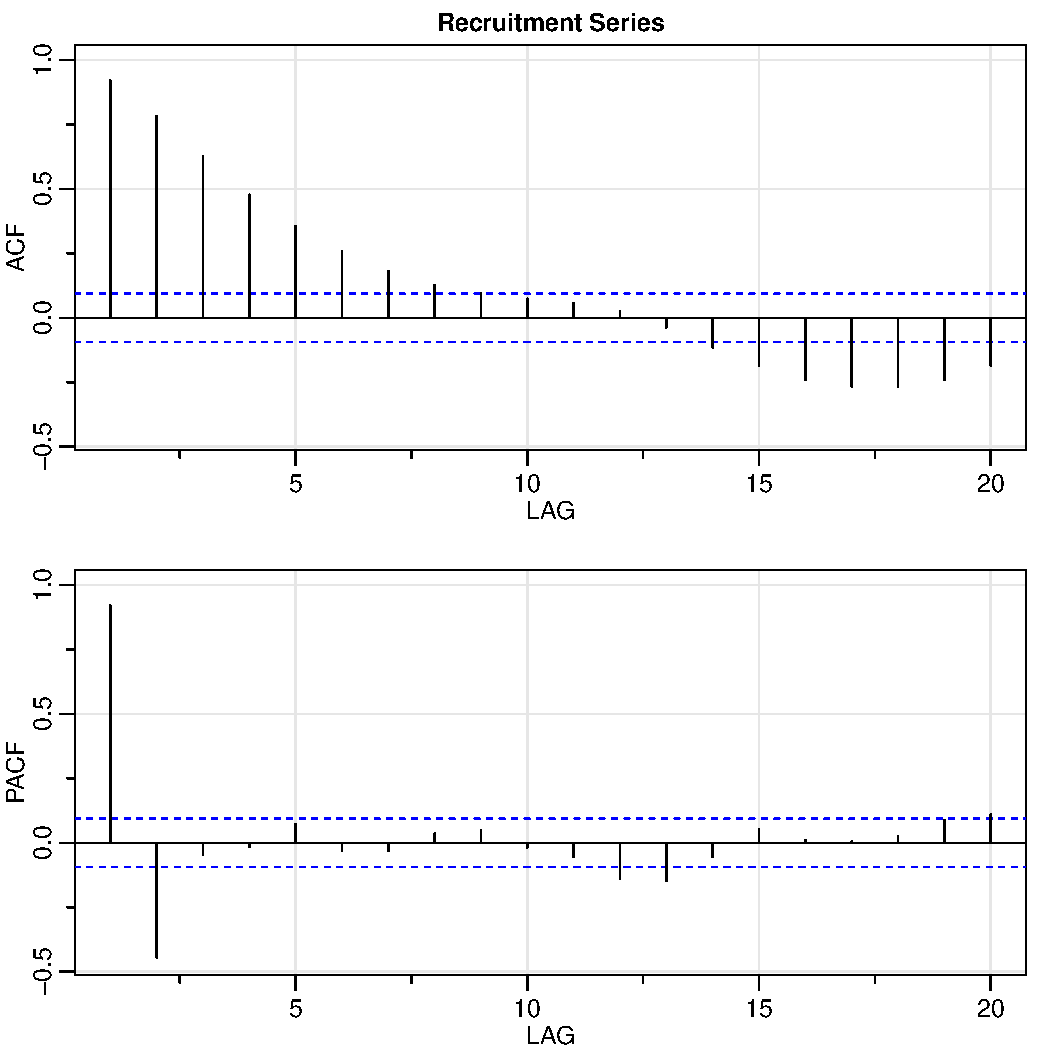
\includegraphics[width=100mm, height=80mm]{recruit.pdf}

\end{frame}

\end{document} 